\documentclass[../main.tex]{subfiles}
 
\begin{document}

\section{Tervezési feladat követelményeinek felállítása}
    A feladatot az Ebay-en vásárolt olcsó mudulok segítségével szerettem volna megvalósítani, amik már a rendelkezésemre álltak. A cél egy olyan áramköri elem megéptése volt, ami viszonylag könnyedén beforrasztható, külső egyenáramú tápellátásről vezérelni tudja a rákapcsolt LED sorokat, és egy cserélhető Wifi modulon keresztül képes az Androidos applikációnkból érkező, általam definiált protokollú, adatok fogadására. Továbbá egy olyan védődoboz tervezése, amivel különböző helyekre lehet majd felszerelni.
    
    \subsection{Rendelkezésre álló hardverek}
        \subsubsection{Wifi modul: ESP8266 - ESP01} %https://www.jayconsystems.com/esp8266-wifi-tranceiver.html
            Az ESP8266 egy olyan IC, ami IoT világnak megfelelően lett tervezve. Képes egy 802.11 típusú hálózaton TCP/IP protokol segítségével kommunikálni. Teljesen címezhető SPI vagy UART segítségével, és hozzáférést ad a GPIO-hoz.\\[12px]
            Néhány tulajdonsága:
            \begin{itemize}
                \item 802.11 b/g/n szabványokat támogat
                \item Wi-Fi Direct (P2P), soft-AP módú működés
                \item integrált TCP/IP protokol
                \item integrált WEP, TKIP, AES motorok
                \item 3.3V DC tápfelszültség
            \end{itemize}
            
            Ennek az IC-nek az ESP01 típusú modulját (Ábra \ref{fig:esp01}) használtam. Körübelül 500 Ft-ért lehet hozzájutni az Ebay-en, és egy 2x4-es csatlakozóval lehet az áramkörünkhöz csatlakoztatni.
            
            \begin{figure}[h!]
                \centering
                    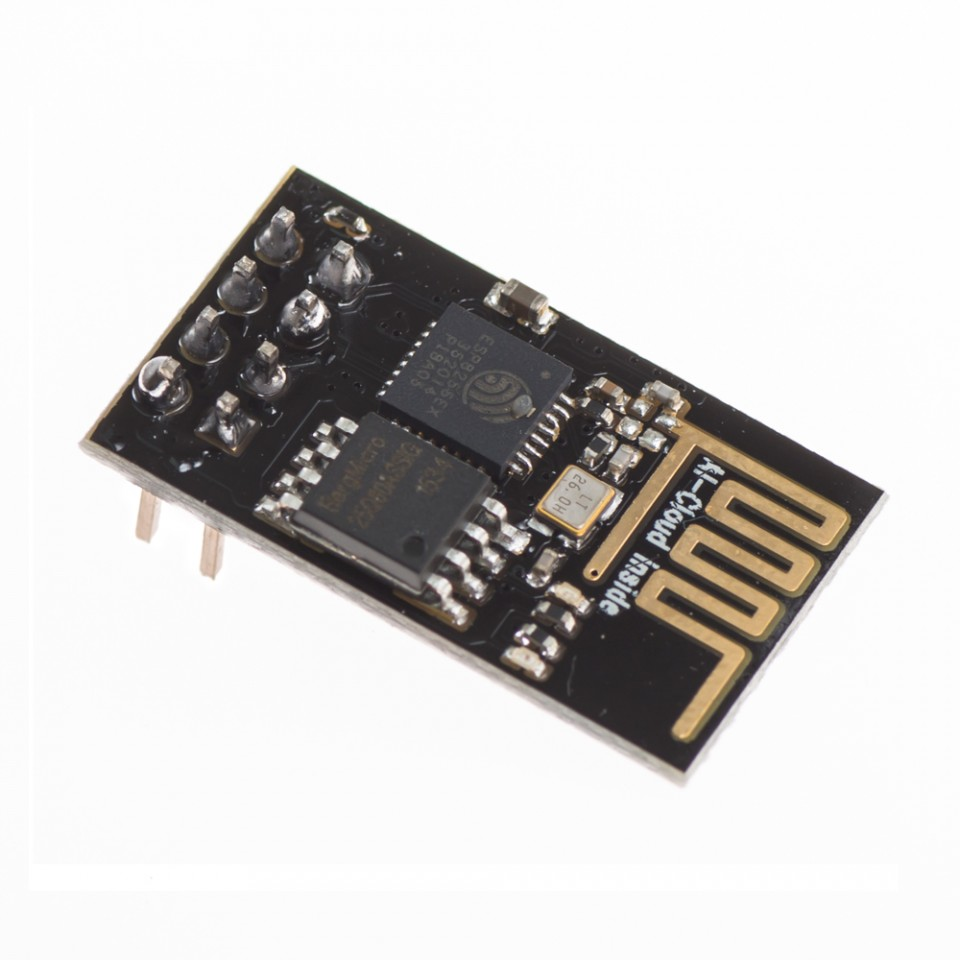
\includegraphics[width=5cm]{resources/pcb_res/esp01.jpg}
                \caption{ESP01-es Wifi Modul}
                \label{fig:esp01}
            \end{figure}
        
        \subsubsection{WS2811-es IC-vel ellátott címezhető LED szalag}
            
            \begin{figure}[h!]
                \centering
                    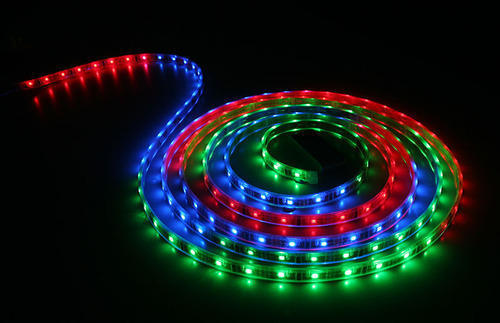
\includegraphics[width=10cm]{resources/pcb_res/ledstrip.jpg}
                \caption{Ebay-ről vásárolt LED szalag //TODO kép frissítése (dummy kép)}
                \label{fig:ledstrip}
            \end{figure}
        
            A WS2811 egy 3 kimeneti csatornás speciális LED meghajtó IC. Egy jelvezetéken küldött 24 bit szélességű bitsorozattal lehet vezérelni 400 vagy 800 Kbps sebességgel. Az IC-ben van belső jelerősítő, hogy egymás után lehessen kötni őket. Az általam vásárolt LED szalagon IC-ként 3[db] RGB LED található, és ezek az IC-k az imént említett módon vannak összekötve. Ezt a felépítést szemlélteti \aref{fig:ledstrip_schematic}.~Ábra.\\[12px]
            
            \begin{figure}[h!] %datasheet ws2811
                \centering
                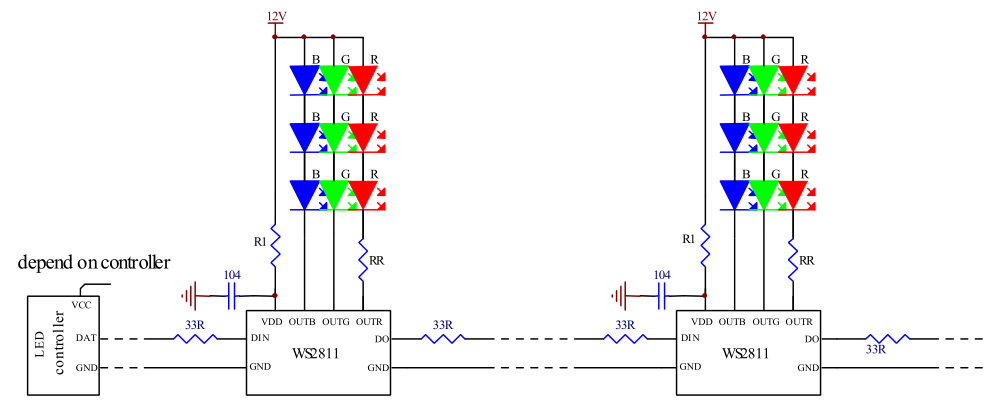
\includegraphics[width=14cm]{resources/pcb_res/ledstrip_schematic.png}
                \caption{Ebay-ről vásárolt LED szalag felépítése}
                \label{fig:ledstrip_schematic}
            \end{figure}
            
            LED szalag tulajdonságai:
            \begin{itemize}
                \item 12V DC tápfeszültség
                \item 1 A maximális áramfelvétel
                \item 5V-os jelvezeték
                \item 5 $m$ hosszú, 150 RGB LED-et tartalmaz
                \item 3 RGB LED/IC
            \end{itemize}
            
        \subsubsection{Mikrovezérlő: STM32F103C8T6}
            Ez a mikrovezérlő az F103-as család tagja, azon belül pedig az a változat aminek 48 lába van (C), 64 Kbyte Flash memóriája van (8), LQFP csomagú (T) és -40-től +85°C-ig működik (6). //ref datasheet
            
            \begin{figure}[h!] % https://hacktronics.co.in/microcontrollers/stm32f103c8t6-cortex-m3-32-bbit-risc-core-72-mhz-microcontroller-lqfp48-package
                \centering
                    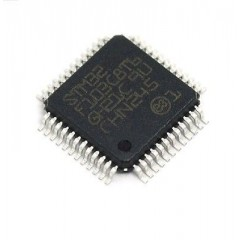
\includegraphics[width=6cm]{resources/pcb_res/stm32f103c8t6.jpg}
                \caption{STM32F103C8T6 típusú mikrovezérlő}
                \label{fig:stm32f103_ic}
            \end{figure}
            
            Egy maximum 72 MHz-es, 32-bit-es ARM Cortex-M3-as processzor a magja, ami a fent említtett Flash és SRAM memória és megannyi más egység (2x A/D konverter, DMA vezérlő 37 I/O port, 7x timer, és 9 kommunikációs interfész) is kiegészít. Számomra az időzítők (PWM generálás, és időzítési feladatok), az UART interfész és a DMA vezérlő játszik fontos szerepet, illetve az A/D konverterek bővítési lehetőségként.
            
            % https://s3-ap-southeast-1.amazonaws.com/a2.datacaciques.com/00/NDAy/17/12/16/9e54ifgdt2zm4pk9/6fec5ff2017d7c73.jpg
            \begin{figure}[h!]
                \centering
                    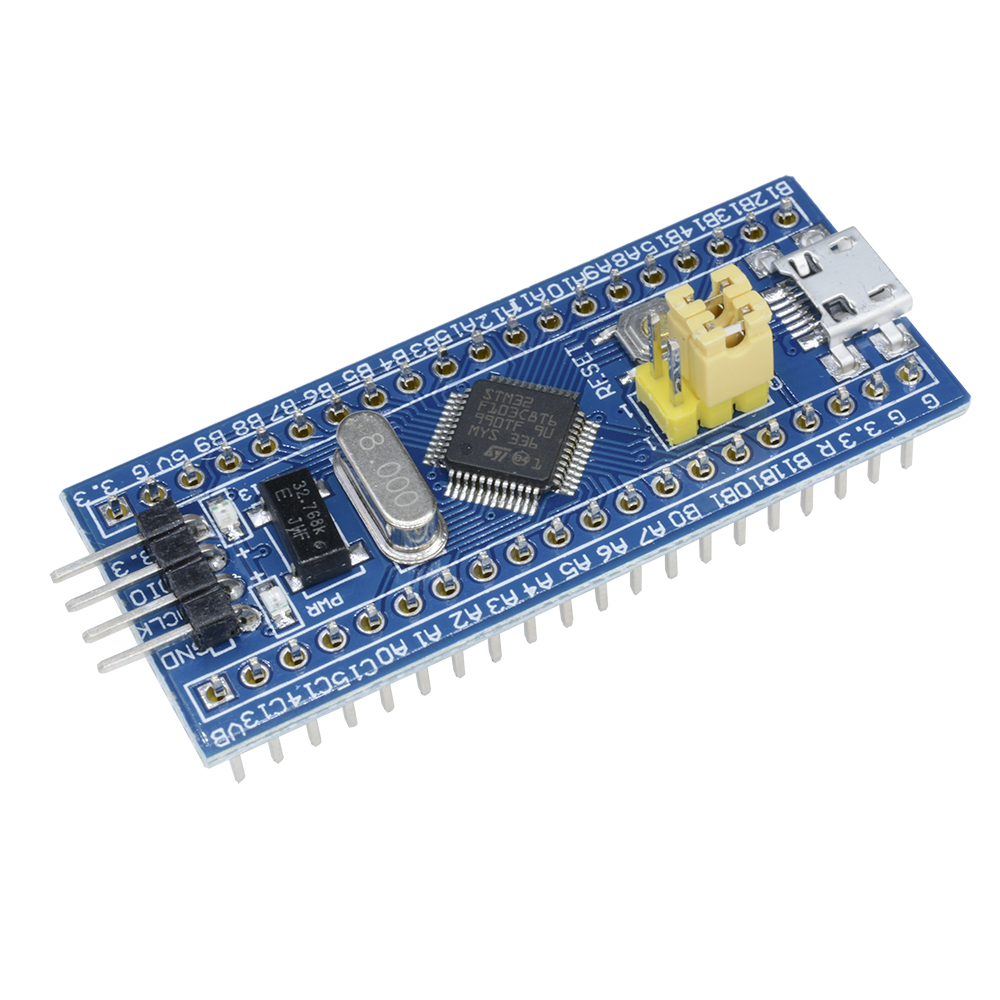
\includegraphics[width=7cm]{resources/pcb_res/stm32f103c8t6_minimum_dev_board.jpg}
                \caption{Ebay-ről vásárolt STM32F103C8T6-es minimum fejlesztői lap}
                \label{fig:stm32f103_dev_board}
            \end{figure}
        
        %\subsubsection{DC/DC konverter prototípus tesztelésénél}
         %A feladat kezdeti megvalósítása során használtam még egy, ugyancsak Ebay-ről rendelt, DC/DC step down konvertert, 
            
    \subsection{Tervezési követelmények összefoglalása}
        \begin{itemize}
            \item Tápfeszültségek
                 \begin{itemize}
                    \item 12V DC tápfeszültség a LED sor számára
                    \item 3,3V DC tápfeszültség a mikrovezérlő és a Wifi-modul számára
                    \item 5V DC tápfeszültség a mikrovezérlőből kijövő 3,3V jelének 5V-sra alakításához
                \end{itemize}
            \item Egyéb
                \begin{itemize}
                    \item rendelkezésre álló modulokból épüljön fel
                    \item legyen minél kisebb, de még kézzel beforrasztható
                \end{itemize}
        \end{itemize}
       
        %A vezérlő NYÁK-om táplálására egy 12V-os, szűrt, egyenáramú tápegységet választottam, mivel így a LED sort közvetlenül a NYÁK-ról meg tudom majd táplálni.   
\end{document}